% Generated by recon/fig-method.mjs --- do not edit by hand.
% Regenerate after any change to domain / grove-core / grove-objective.
\documentclass[tikz,border=2pt]{standalone}
\usepackage{amsmath,amssymb}
\usetikzlibrary{arrows.meta}
\definecolor{banditcol}{HTML}{2A78D6}
\definecolor{wifecol}{HTML}{EB6834}
\definecolor{samuraicol}{HTML}{1BAF7A}
\definecolor{inkcol}{HTML}{0B0B0B}
\definecolor{okcol}{HTML}{1B7A4A}
\definecolor{nocol}{HTML}{B03A2E}
\begin{document}
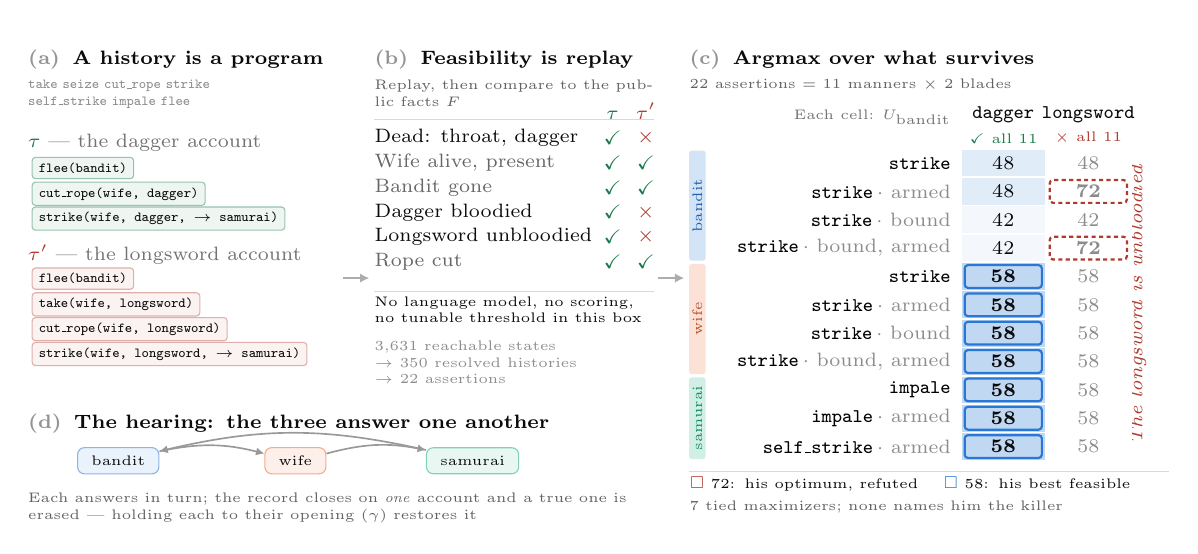
\begin{tikzpicture}[font=\small, inner sep=0pt]
  %% fixed canvas, so the float width does not drift between regenerations
  \path (0,0.28) rectangle (14.5,-6.05);
  \draw[-{Latex[length=3.4pt,width=3.4pt]}, black!32, line width=0.7pt] (4.01,-2.9) -- (4.340000000000001,-2.9);
  \draw[-{Latex[length=3.4pt,width=3.4pt]}, black!32, line width=0.7pt] (8.01,-2.9) -- (8.34,-2.9);

  \node[anchor=north west, font=\scriptsize\bfseries, text=inkcol, align=left, text width=3.95cm] at (0,0) {\textcolor{black!42}{(a)}\, A history is a program};
  \node[anchor=north west, font=\tiny\ttfamily, text=black!45, align=left, text width=3.95cm] at (0,-0.38) {take~seize~cut\_rope~strike\\self\_strike~impale~flee};
  \node[anchor=north west, font=\scriptsize, text=okcol] at (0,-1.06) {$\tau$ \textcolor{black!55}{--- the dagger account}};
  \node[anchor=north west, draw=okcol!45, line width=0.4pt, rounded corners=1.2pt, fill=okcol!7, inner xsep=2.4pt, inner ysep=1.9pt, font=\tiny\ttfamily, text=inkcol] at (0.05,-1.36) {flee(bandit)};
  \node[anchor=north west, draw=okcol!45, line width=0.4pt, rounded corners=1.2pt, fill=okcol!7, inner xsep=2.4pt, inner ysep=1.9pt, font=\tiny\ttfamily, text=inkcol] at (0.05,-1.675) {cut\_rope(wife, dagger)};
  \node[anchor=north west, draw=okcol!45, line width=0.4pt, rounded corners=1.2pt, fill=okcol!7, inner xsep=2.4pt, inner ysep=1.9pt, font=\tiny\ttfamily, text=inkcol] at (0.05,-1.99) {strike(wife, dagger, $\to$ samurai)};
  \node[anchor=north west, font=\scriptsize, text=nocol] at (0,-2.4650000000000003) {$\tau'$ \textcolor{black!55}{--- the longsword account}};
  \node[anchor=north west, draw=nocol!40, line width=0.4pt, rounded corners=1.2pt, fill=nocol!6, inner xsep=2.4pt, inner ysep=1.9pt, font=\tiny\ttfamily, text=inkcol] at (0.05,-2.765) {flee(bandit)};
  \node[anchor=north west, draw=nocol!40, line width=0.4pt, rounded corners=1.2pt, fill=nocol!6, inner xsep=2.4pt, inner ysep=1.9pt, font=\tiny\ttfamily, text=inkcol] at (0.05,-3.08) {take(wife, longsword)};
  \node[anchor=north west, draw=nocol!40, line width=0.4pt, rounded corners=1.2pt, fill=nocol!6, inner xsep=2.4pt, inner ysep=1.9pt, font=\tiny\ttfamily, text=inkcol] at (0.05,-3.395) {cut\_rope(wife, longsword)};
  \node[anchor=north west, draw=nocol!40, line width=0.4pt, rounded corners=1.2pt, fill=nocol!6, inner xsep=2.4pt, inner ysep=1.9pt, font=\tiny\ttfamily, text=inkcol] at (0.05,-3.71) {strike(wife, longsword, $\to$ samurai)};
  \node[anchor=north west, font=\scriptsize\bfseries, text=inkcol, align=left, text width=3.55cm] at (4.4,0) {\textcolor{black!42}{(b)}\, Feasibility is replay};
  \node[anchor=north west, font=\tiny, text=black!62, align=left, text width=3.55cm] at (4.4,-0.38) {Replay, then compare to the public facts $F$};
  \node[anchor=south, font=\scriptsize, text=okcol] at (7.43,-0.89) {$\tau$};
  \node[anchor=south, font=\scriptsize, text=nocol] at (7.8500000000000005,-0.89) {$\tau'$};
  \draw[gray!30, line width=0.4pt] (4.4,-0.89) -- (7.95,-0.89);
  \node[anchor=west, font=\scriptsize, text=inkcol] at (4.4,-1.12) {Dead: throat, dagger};
  \node[font=\scriptsize, text=okcol] at (7.43,-1.12) {$\checkmark$};
  \node[font=\scriptsize, text=nocol] at (7.8500000000000005,-1.12) {$\times$};
  \node[anchor=west, font=\scriptsize, text=black!60] at (4.4,-1.435) {Wife alive, present};
  \node[font=\scriptsize, text=okcol] at (7.43,-1.435) {$\checkmark$};
  \node[font=\scriptsize, text=okcol] at (7.8500000000000005,-1.435) {$\checkmark$};
  \node[anchor=west, font=\scriptsize, text=black!60] at (4.4,-1.75) {Bandit gone};
  \node[font=\scriptsize, text=okcol] at (7.43,-1.75) {$\checkmark$};
  \node[font=\scriptsize, text=okcol] at (7.8500000000000005,-1.75) {$\checkmark$};
  \node[anchor=west, font=\scriptsize, text=inkcol] at (4.4,-2.065) {Dagger bloodied};
  \node[font=\scriptsize, text=okcol] at (7.43,-2.065) {$\checkmark$};
  \node[font=\scriptsize, text=nocol] at (7.8500000000000005,-2.065) {$\times$};
  \node[anchor=west, font=\scriptsize, text=inkcol] at (4.4,-2.38) {Longsword unbloodied};
  \node[font=\scriptsize, text=okcol] at (7.43,-2.38) {$\checkmark$};
  \node[font=\scriptsize, text=nocol] at (7.8500000000000005,-2.38) {$\times$};
  \node[anchor=west, font=\scriptsize, text=black!60] at (4.4,-2.695) {Rope cut};
  \node[font=\scriptsize, text=okcol] at (7.43,-2.695) {$\checkmark$};
  \node[font=\scriptsize, text=okcol] at (7.8500000000000005,-2.695) {$\checkmark$};
  \draw[gray!30, line width=0.4pt] (4.4,-3.07) -- (7.95,-3.07);
  \node[anchor=north west, font=\tiny, text=inkcol, align=left, text width=3.55cm] at (4.4,-3.13) {No language model, no scoring,\\no tunable threshold in this box};
  \node[anchor=north west, font=\tiny, text=black!45, align=left, text width=3.55cm] at (4.4,-3.69) {3,631 reachable states\\$\to$ 350 resolved histories\\$\to$ 22 assertions};
  \node[anchor=north west, font=\scriptsize\bfseries, text=inkcol, align=left, text width=6.1cm] at (8.4,0) {\textcolor{black!42}{(c)}\, Argmax over what survives};
  \node[anchor=north west, font=\tiny, text=black!62, align=left, text width=6.1cm] at (8.4,-0.36) {22 assertions $=$ 11 manners $\times$ 2 blades};
  \fill[nocol!6] (12.930000000000003,-1.26) rectangle (14.010000000000002,-5.22);
  \node[anchor=south, font=\scriptsize\ttfamily, text=inkcol] at (12.39,-0.94) {dagger};
  \node[anchor=south, font=\tiny, text=okcol] at (12.39,-1.2) {$\checkmark$ all 11};
  \node[anchor=south, font=\scriptsize\ttfamily, text=inkcol] at (13.470000000000002,-0.94) {longsword};
  \node[anchor=south, font=\tiny, text=nocol] at (13.470000000000002,-1.2) {$\times$ all 11};
  \node[anchor=south east, font=\tiny, text=black!55] at (11.730000000000002,-0.96) {Each cell: $U_{\mathrm{bandit}}$};
  \node[rotate=90, anchor=south, font=\scriptsize\itshape, text=nocol] at (14.21,-3.2399999999999998) {The longsword is unbloodied};
  \fill[banditcol!20, rounded corners=1pt] (8.4,-1.28) rectangle (8.610000000000001,-2.68);
  \node[rotate=90, font=\tiny, text=banditcol!80!black] at (8.505,-1.98) {bandit};
  \fill[wifecol!20, rounded corners=1pt] (8.4,-2.72) rectangle (8.610000000000001,-4.12);
  \node[rotate=90, font=\tiny, text=wifecol!80!black] at (8.505,-3.42) {wife};
  \fill[samuraicol!20, rounded corners=1pt] (8.4,-4.159999999999999) rectangle (8.610000000000001,-5.2);
  \node[rotate=90, font=\tiny, text=samuraicol!80!black] at (8.505,-4.68) {samurai};
  \node[anchor=east, font=\scriptsize] at (11.730000000000002,-1.44) {{\ttfamily strike}};
  \node[draw=white, line width=0.6pt, fill=banditcol!14, minimum width=1.08cm, minimum height=0.36cm, inner sep=0pt, font=\scriptsize, text=inkcol] at (12.39,-1.44) {48};
  \node[draw=white, line width=0.6pt, fill=black!0, minimum width=1.08cm, minimum height=0.36cm, inner sep=0pt, font=\scriptsize, text=black!45] at (13.470000000000002,-1.44) {48};
  \node[anchor=east, font=\scriptsize] at (11.730000000000002,-1.8) {{\ttfamily strike}\,\textcolor{black!45}{$\cdot$ armed}};
  \node[draw=white, line width=0.6pt, fill=banditcol!14, minimum width=1.08cm, minimum height=0.36cm, inner sep=0pt, font=\scriptsize, text=inkcol] at (12.39,-1.8) {48};
  \node[draw=white, line width=0.6pt, fill=black!0, minimum width=1.08cm, minimum height=0.36cm, inner sep=0pt, font=\scriptsize, text=black!45] at (13.470000000000002,-1.8) {\bfseries 72};
  \draw[draw=nocol, line width=0.8pt, dash pattern=on 1.5pt off 1.2pt, rounded corners=1.2pt] (12.980000000000004,-1.945) rectangle (13.96,-1.655);
  \node[anchor=east, font=\scriptsize] at (11.730000000000002,-2.16) {{\ttfamily strike}\,\textcolor{black!45}{$\cdot$ bound}};
  \node[draw=white, line width=0.6pt, fill=banditcol!5, minimum width=1.08cm, minimum height=0.36cm, inner sep=0pt, font=\scriptsize, text=inkcol] at (12.39,-2.16) {42};
  \node[draw=white, line width=0.6pt, fill=black!0, minimum width=1.08cm, minimum height=0.36cm, inner sep=0pt, font=\scriptsize, text=black!45] at (13.470000000000002,-2.16) {42};
  \node[anchor=east, font=\scriptsize] at (11.730000000000002,-2.52) {{\ttfamily strike}\,\textcolor{black!45}{$\cdot$ bound, armed}};
  \node[draw=white, line width=0.6pt, fill=banditcol!5, minimum width=1.08cm, minimum height=0.36cm, inner sep=0pt, font=\scriptsize, text=inkcol] at (12.39,-2.52) {42};
  \node[draw=white, line width=0.6pt, fill=black!0, minimum width=1.08cm, minimum height=0.36cm, inner sep=0pt, font=\scriptsize, text=black!45] at (13.470000000000002,-2.52) {\bfseries 72};
  \draw[draw=nocol, line width=0.8pt, dash pattern=on 1.5pt off 1.2pt, rounded corners=1.2pt] (12.980000000000004,-2.665) rectangle (13.96,-2.375);
  \node[anchor=east, font=\scriptsize] at (11.730000000000002,-2.8800000000000003) {{\ttfamily strike}};
  \node[draw=white, line width=0.6pt, fill=banditcol!29, minimum width=1.08cm, minimum height=0.36cm, inner sep=0pt, font=\scriptsize, text=inkcol] at (12.39,-2.8800000000000003) {\bfseries 58};
  \draw[draw=banditcol, line width=0.8pt, rounded corners=1.2pt] (11.900000000000002,-3.0250000000000004) rectangle (12.879999999999999,-2.7350000000000003);
  \node[draw=white, line width=0.6pt, fill=black!0, minimum width=1.08cm, minimum height=0.36cm, inner sep=0pt, font=\scriptsize, text=black!45] at (13.470000000000002,-2.8800000000000003) {58};
  \node[anchor=east, font=\scriptsize] at (11.730000000000002,-3.2399999999999998) {{\ttfamily strike}\,\textcolor{black!45}{$\cdot$ armed}};
  \node[draw=white, line width=0.6pt, fill=banditcol!29, minimum width=1.08cm, minimum height=0.36cm, inner sep=0pt, font=\scriptsize, text=inkcol] at (12.39,-3.2399999999999998) {\bfseries 58};
  \draw[draw=banditcol, line width=0.8pt, rounded corners=1.2pt] (11.900000000000002,-3.385) rectangle (12.879999999999999,-3.0949999999999998);
  \node[draw=white, line width=0.6pt, fill=black!0, minimum width=1.08cm, minimum height=0.36cm, inner sep=0pt, font=\scriptsize, text=black!45] at (13.470000000000002,-3.2399999999999998) {58};
  \node[anchor=east, font=\scriptsize] at (11.730000000000002,-3.6) {{\ttfamily strike}\,\textcolor{black!45}{$\cdot$ bound}};
  \node[draw=white, line width=0.6pt, fill=banditcol!29, minimum width=1.08cm, minimum height=0.36cm, inner sep=0pt, font=\scriptsize, text=inkcol] at (12.39,-3.6) {\bfseries 58};
  \draw[draw=banditcol, line width=0.8pt, rounded corners=1.2pt] (11.900000000000002,-3.745) rectangle (12.879999999999999,-3.455);
  \node[draw=white, line width=0.6pt, fill=black!0, minimum width=1.08cm, minimum height=0.36cm, inner sep=0pt, font=\scriptsize, text=black!45] at (13.470000000000002,-3.6) {58};
  \node[anchor=east, font=\scriptsize] at (11.730000000000002,-3.9600000000000004) {{\ttfamily strike}\,\textcolor{black!45}{$\cdot$ bound, armed}};
  \node[draw=white, line width=0.6pt, fill=banditcol!29, minimum width=1.08cm, minimum height=0.36cm, inner sep=0pt, font=\scriptsize, text=inkcol] at (12.39,-3.9600000000000004) {\bfseries 58};
  \draw[draw=banditcol, line width=0.8pt, rounded corners=1.2pt] (11.900000000000002,-4.105) rectangle (12.879999999999999,-3.8150000000000004);
  \node[draw=white, line width=0.6pt, fill=black!0, minimum width=1.08cm, minimum height=0.36cm, inner sep=0pt, font=\scriptsize, text=black!45] at (13.470000000000002,-3.9600000000000004) {58};
  \node[anchor=east, font=\scriptsize] at (11.730000000000002,-4.319999999999999) {{\ttfamily impale}};
  \node[draw=white, line width=0.6pt, fill=banditcol!29, minimum width=1.08cm, minimum height=0.36cm, inner sep=0pt, font=\scriptsize, text=inkcol] at (12.39,-4.319999999999999) {\bfseries 58};
  \draw[draw=banditcol, line width=0.8pt, rounded corners=1.2pt] (11.900000000000002,-4.464999999999999) rectangle (12.879999999999999,-4.175);
  \node[draw=white, line width=0.6pt, fill=black!0, minimum width=1.08cm, minimum height=0.36cm, inner sep=0pt, font=\scriptsize, text=black!45] at (13.470000000000002,-4.319999999999999) {58};
  \node[anchor=east, font=\scriptsize] at (11.730000000000002,-4.68) {{\ttfamily impale}\,\textcolor{black!45}{$\cdot$ armed}};
  \node[draw=white, line width=0.6pt, fill=banditcol!29, minimum width=1.08cm, minimum height=0.36cm, inner sep=0pt, font=\scriptsize, text=inkcol] at (12.39,-4.68) {\bfseries 58};
  \draw[draw=banditcol, line width=0.8pt, rounded corners=1.2pt] (11.900000000000002,-4.824999999999999) rectangle (12.879999999999999,-4.535);
  \node[draw=white, line width=0.6pt, fill=black!0, minimum width=1.08cm, minimum height=0.36cm, inner sep=0pt, font=\scriptsize, text=black!45] at (13.470000000000002,-4.68) {58};
  \node[anchor=east, font=\scriptsize] at (11.730000000000002,-5.039999999999999) {{\ttfamily self\_strike}\,\textcolor{black!45}{$\cdot$ armed}};
  \node[draw=white, line width=0.6pt, fill=banditcol!29, minimum width=1.08cm, minimum height=0.36cm, inner sep=0pt, font=\scriptsize, text=inkcol] at (12.39,-5.039999999999999) {\bfseries 58};
  \draw[draw=banditcol, line width=0.8pt, rounded corners=1.2pt] (11.900000000000002,-5.184999999999999) rectangle (12.879999999999999,-4.895);
  \node[draw=white, line width=0.6pt, fill=black!0, minimum width=1.08cm, minimum height=0.36cm, inner sep=0pt, font=\scriptsize, text=black!45] at (13.470000000000002,-5.039999999999999) {58};
  \draw[gray!30, line width=0.4pt] (8.4,-5.359999999999999) -- (14.5,-5.359999999999999);
  \node[anchor=north west, font=\tiny, text=inkcol, align=left, text width=6.1cm] at (8.4,-5.42) {\textcolor{nocol}{$\square$}~72: his optimum, refuted \quad \textcolor{banditcol}{$\square$}~58: his best feasible};
  \node[anchor=north west, font=\tiny, text=black!62, align=left, text width=6.1cm] at (8.4,-5.72) {7 tied maximizers; none names him the killer};
  \node[anchor=north west, font=\scriptsize\bfseries, text=inkcol, align=left, text width=7.8500000000000005cm] at (0,-4.62) {\textcolor{black!42}{(d)}\, The hearing: the three answer one another};
  \node[draw=banditcol!55, fill=banditcol!10, rounded corners=2.5pt, inner xsep=5pt, inner ysep=3pt, font=\tiny, text=inkcol] (h0) at (1.15,-5.22) {bandit};
  \node[draw=wifecol!55, fill=wifecol!10, rounded corners=2.5pt, inner xsep=5pt, inner ysep=3pt, font=\tiny, text=inkcol] (h1) at (3.4,-5.22) {wife};
  \node[draw=samuraicol!55, fill=samuraicol!10, rounded corners=2.5pt, inner xsep=5pt, inner ysep=3pt, font=\tiny, text=inkcol] (h2) at (5.65,-5.22) {samurai};
  \draw[-{Latex[length=3pt,width=3pt]}, black!40, line width=0.6pt] (h0) to[bend left=13] (h1);
  \draw[-{Latex[length=3pt,width=3pt]}, black!40, line width=0.6pt] (h1) to[bend left=13] (h2);
  \draw[-{Latex[length=3pt,width=3pt]}, black!40, line width=0.6pt] (h2) to[bend right=13] (h0);
  \node[anchor=north west, font=\tiny, text=black!62, align=left, text width=7.8500000000000005cm] at (0,-5.62) {Each answers in turn; the record closes on \emph{one} account and a true one is erased --- holding each to their opening ($\gamma$) restores it};

\end{tikzpicture}
\end{document}
